\documentclass[11pt]{article}


%%%%%%%%%%%%%%%
\def\Type{ApplicationDJ}
\def\TypeNum{Pre-class for Application Day: Gradient Descent Method}
\def\TypeTitle{Gradient Descent}
\def\Semester{Fall 2025}
\def\Course{Math 1190/1210}
%\def\Targets{{\bf\color{Goldenrod}AD1}}
\def\desmosClassCode{{\bf ZAJ$3$AZ}}
\usepackage{preambleDJ}
\usepackage{graphicx}
\usepackage{footnote}
\usepackage{tikz}
\usepackage{pgfplots}
\usepackage[colorlinks=true, linkcolor=blue, urlcolor=blue]{hyperref}
%\pgfplotsset{compat=1.18}  % adjust to your version
\makesavenoteenv{minipage}
\begin{document}
%!TEX TS-program = xelatex
%!TEX encoding = UTF-8 Unicode



\pagestyle{otherpages}
\thispagestyle{firstpage}
\vspace*{.65in}


%!TEX TS-program = xelatex
%!TEX encoding = UTF-8 Unicode



%If Ada Lovelace\footnote{\url{https://en.wikipedia.org/wiki/Ada_Lovelace}} is the ``mother of programming" then 
{\bf Introduction}\\

\noindent
\begin{minipage}[c]{0.35\textwidth}
    \centering
    
\includegraphics[width=\linewidth]{Spring 2026/ApplicationDays/GradientDescent/images/feiFeiLiWiredCropped.png}
    Fei-Fei Li is known as the ``godmother of A.I'' for her groundbreaking contributions in computer vision and deep learning and as the creator of ImageNet\footnote{
See ``Godmother of A.I." Fei-Fei Li on technology development: ``The power lies within people" at \url{https://www.cbsnews.com/news/godmother-of-a-i-on-technology-development-fei-fei-li/}\\
or Britannica at \url{https://www.britannica.com/biography/Fei-Fei-Li}, The Guardian \href{https://www.theguardian.com/technology/2023/nov/05/ai-pioneer-fei-fei-li-im-more-concerned-about-the-risks-that-are-here-and-now}{\underline{here}} or \url{https://en.wikipedia.org/wiki/Fei-Fei_Li}
}.
\end{minipage}
\hspace{0.02\textwidth}
\begin{minipage}[c]{0.63\textwidth}


\vspace{1em}

In this application, we will be exploring how the tools of calculus can be applied in machine learning. \textit{Machine learning} refers to computer programs for which the outputs mimic patterns in a specific dataset, but without these patterns being explicitly described in the programming. This field powers much of modern artificial intelligence. For example, while generative AI's like ChatGPT can produce coherent English sentences, their code does not contain the rules of English grammar and syntax; rather, they ``learn" these rules autonomously by processing large amounts of examples. 

This learning process can be viewed as an optimization problem in the following way:
\begin{itemize}
    \item The algorithm to generate new outputs contains many \textit{parameters,} which each influence the outputs generated.
    \item Once the parameters have been chosen, the outputs of the algorithm are compared against the data set. The algorithm is then given a \textit{loss} score, where a smaller loss indicates a closer match to the data.
    \item The \textit{loss function} takes the parameters as input and gives the loss of the corresponding algorithm as an output. The optimization problem is then to find the parameter set which minimizes the loss function.
\end{itemize}
\end{minipage}
\newpage


















%%%%%%%%%%%%%%%%%%%%%%%%%%%%%%%%%%%%%%%%%%%%%%%%%%%%%%%%%%%%%%%%%%%%%%%%%%%%%%%%%%%%%%%%%%%%%%%%%%%%%%%%%%%%%%%%%%%%%%%%%%%%%%%%%%%%%%%%%%%%%%%%%%%%%%%%%%%%%%%%%%%%%%%%%%%%%%%%%%%%%%%%%%%%%%%%%%%%%%%%%%%%%%%%%%%%%%%%%%%%

Unfortunately, this optimization problem is usually much harder than the ones we've seen in this class so far. One big difference is the number of inputs: every function we've seen has had just one input $x$, while machine learning models can have billions of parameters or more. This means it is very hard to visualize or graph the loss function. Another issue is that the function itself is so complicated that we cannot simply write down the derivative and find critical numbers in the usual way.

In this situation, one of the tools we can use is \textit{gradient descent}. Gradient descent is a method used for optimization which only requires us to be able to evaluate a function and its derivative at individual points in the domain. Throughout this worksheet, we will develop the ideas of gradient descent for a single-variable function $f(x)$.

{\bf Example 1: Function and Derivative}\\

Suppose that we evaluate our function and its derivative at $x=1$ to get that $f(1) = 1$ and $f'(1) = 2$.

\begin{enumerate}
\item Write down the equation of the line tangent to $f(x)$ at the point $(1,1)$:
\[
    y = \rule{2cm}{0.4pt}
\]
\end{enumerate}

A small segment of the tangent line is sketched below in red, along with an example in blue of what $f(x)$ might look like near the point $(1,1)$.

\begin{center}
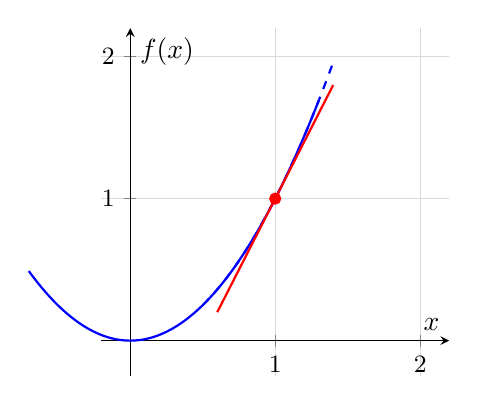
\begin{tikzpicture}
\begin{axis}[
    height = 6cm,
    width = 6cm,
    axis lines=middle,
    xlabel=$x$, ylabel=$f(x)$,
    xmin=-0.2, xmax=2.2,
    ymin=-0.25, ymax=2.2,
    xtick={0,1,2},
    ytick={0,1,2},
    grid=both,              % add grid lines
    grid style={gray!30},   % light gray grid
    tick label style={font=\small}, % smaller labels
    enlargelimits=false,
    clip=false
]

% f(x) = x^2
\addplot [domain=-0.7:1.3, samples=100, blue, thick] {x^2};
\addplot [domain=0.5:1.4, samples=100, blue, thick, dashed] {x^2};

% Tangent at x=3: f'(3) = 6
\addplot [domain=0.6:1.4, red, thick] {2*(x-1)+1};

% Mark the point (3,9)
\addplot[only marks, mark=*, red] coordinates {(1,1)};
% \node[below right] at (axis cs:1,1) {$(1,1)$};

\end{axis}
\end{tikzpicture}
\end{center}

Call the $x$-value we're currently examining $x_1=1$. We want to choose a new guess $x_2$ which is closer to the minimum of $f(x)$.
From this picture, we can see that since $f'(x_1)>0$, if we pick $x_2 < x_1$ then hopefully  $f(x_2)$ is closer to the minimum. But how much smaller should we make $x_2$? If we change our guess too much, we may overshoot the minimum, but if we change it too little we won't make much progress towards finding the minimum. 

The formula we will use to update our guess is this:
\[
    x_2 = x_1 - \alpha f'(x_1),
\]
where $\alpha$ is some positive constant.
\begin{enumerate}
    \item[2.]  Using $\alpha = 0.1$, compute $x_2$ in our example.
    \[
        x_2 = \rule{2cm}{0.4pt}
    \]
\end{enumerate}
\newpage
This formula makes sense because:
\begin{itemize}
    \item If $f'(x_0)>0$, this moves our guess to the left, just like we wanted. If $f'(x_0) < 0$, this moves our guess to the right.
    \item If $f'(x_0)$ is close to zero, then we're probably close to the minimum and our guess won't move much. If $f'(x_0)$ is large, then the guess will change significantly.
    \item Adjusting the constant $\alpha$ allows us to fine-tune the gradient descent process, either speeding it up or making sure we don't overshoot the minimum.
\end{itemize}
We can then use $f'(x_2)$ to make a new guess $x_3$, use $f'(x_3)$ to make a new guess $x_4$, and so on and so forth until we are confident our guess is close to the minimum.
\begin{figure}[h!]
\centering
\begin{minipage}{0.45\textwidth}
\centering
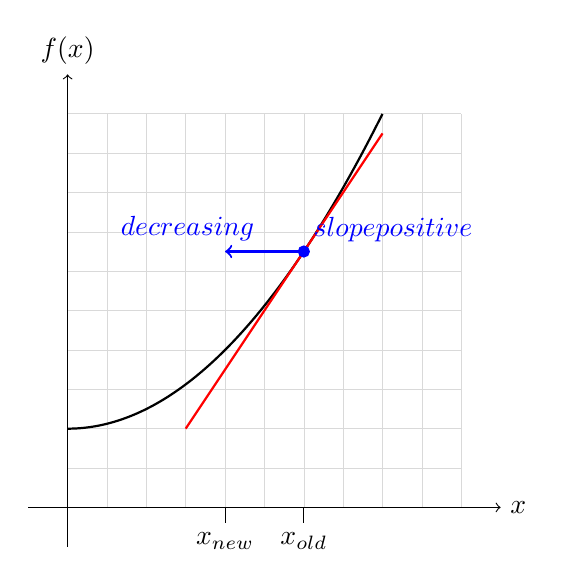
\begin{tikzpicture}[scale=1.0]
    % grid
    \draw[step=0.5, gray!30, very thin] (0,0) grid (5,5);
    
    % axes
    \draw[->] (-0.5,0) -- (5.5,0) node[right] {$x$};
    \draw[->] (0,-0.5) -- (0,5.5) node[above] {$f(x)$};
    
    % function
    \draw[thick, domain=0:4, samples=100, smooth] plot (\x,{0.25*\x*\x+1});
    
    % tangent line through x=3
    \draw[red, thick, domain=1.5:4] plot (\x,{1.5*\x -1.25}); % tangent using slope f'(3)=3
    
    % point on curve
    \filldraw[blue] (3,3.25) circle (2pt) node[above right] {$\text{slope positive}$};
    
    % gradient descent arrow
    \draw[->, thick, blue] (3,3.25) -- (2,3.25) node[midway, above left] {$\text{decreasing }$};
    
    % x labels
    \draw (3,0) -- (3,-0.2) node[below] {$x_\text{old}$};
    \draw (2,0) -- (2,-0.2) node[below] {$x_\text{new}$};
\end{tikzpicture}
\caption*{Slope $f'(x_\text{old})>0$: move left along $x$ to decrease $f(x)$.}
\end{minipage}
\hfill
\begin{minipage}{0.45\textwidth}
\centering
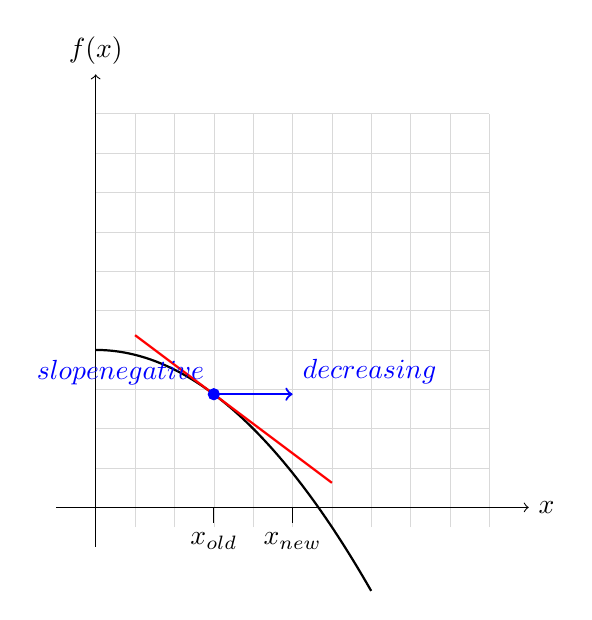
\begin{tikzpicture}[scale=1.0]
    % grid
    \draw[step=0.5, gray!30, very thin] (0,-0.25) grid (5,5);
    
    % axes
    \draw[->] (-0.5,0) -- (5.5,0) node[right] {$x$};
    \draw[->] (0,-0.5) -- (0,5.5) node[above] {$f(x)$};
    
    % function
    \draw[thick, domain=0:3.5, samples=100, smooth] plot (\x,{-0.25*\x*\x+2});
    
    % tangent line through x=1.5
    \draw[red, thick, domain=0.5:3] plot (\x,{-0.75*\x + 2.5625}); % tangent f'(1.5)=1.5
    
    % point on curve
    \filldraw[blue] (1.5,1.4375) circle (2pt) node[above left] {$\text{slope negative}$};
    
    % gradient descent arrow
    \draw[->, thick, blue] (1.5,1.4375) -- (2.5,1.4375) node[above right] {$\text{decreasing}$};
    
    % x labels
    \draw (1.5,0) -- (1.5,-0.2) node[below] {$x_\text{old}$};
    \draw (2.5,0) -- (2.5,-0.2) node[below] {$x_\text{new}$};
\end{tikzpicture}
\caption*{Slope $f'(x_\text{old})<0$: move right along $x$ to decrease $f(x)$.}
\end{minipage}
\end{figure}

\newpage
{\bf Gradient Descent Algorithm}\\

\enum{

\item Let's apply gradient descent to $f(x) = x^4 - 2x^2 + 1$ with $x_1 = 2$ and $\alpha = 0.02$. You may need a calculator.

\enum{
\item Compute $f'(x)$.
\vspace{2cm}
\item Evaluate $f'(x_1)$, and use this to compute a new guess $x_2$.
\vspace{2cm}
\item Evaluate $f'(x_2)$, and use this to compute a new guess $x_3$.
\vspace{2cm}
\item Using our usual optimization tools, where are the local minima of $f(x)$? Which minimum, if any, do our guesses seem to be approaching?
\vspace{4cm}
}
}

\newpage
\section*{Gradient Descent Exploration Activity}

Now open the Gradient Descent app found here: \href{https://woodword0-gradientdescentapplication.hf.space/}{Open the Gradient Descent App}


\begin{itemize}
    \item Select a function from the drop down menu
    \item Try different starting points $x_0$
    \item Try different learning rates $\alpha$
    \item Observe the sequence of points
\end{itemize}

\textbf{Answer the following questions:}

\begin{enumerate}

    \item For $f(x) = x^2$:
    \begin{itemize}
        \item Does gradient descent always find the minimum?
         \vspace{2cm}
        
        \item What happens if $\alpha$ is very large?
    \end{itemize}
    \vspace{2cm}

    \item For $f(x) = e^x - x$:
    \begin{itemize}
        \item Does the method converge to the same point from different starting values?
        \vspace{2cm}
        
        \item What do you notice about the slope near the minimum?
    \end{itemize}
    \vspace{2cm}

    \item For $f(x) = x^4 - 2x^2 + 1$:
    \begin{itemize}
        \item How many minimums does this function have?
         \vspace{2cm}
        
        \item Does gradient descent always find the same one?
         \vspace{2cm}
        
        \item How does the starting point affect the result?
    \end{itemize}

\end{enumerate}


\end{document}